% !TEX program = xelatex

\documentclass{resume}
\usepackage{verbatim}
\usepackage{graphicx}
\usepackage{tabu}
\usepackage{multirow}
\usepackage{zh_CN-Adobefonts_external} % Simplified Chinese Support using external fonts (./fonts/zh_CN-Adobe/)
%\usepackage{zh_CN-Adobefonts_internal} % Simplified Chinese Support using system fonts

\begin{document}
\pagenumbering{gobble} % suppress displaying page number

\Large{
  \begin{tabu}{ clr }
   %\multirow{5}{1in}{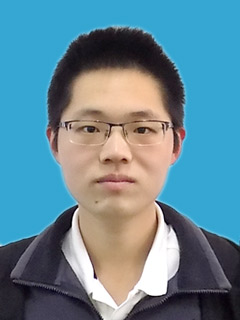
\includegraphics[width=0.88in, height=1.15in]{avatar}}
    & \scshape{贾臻玮} & \pbar{C++}{0.75} \\
    & \email{manout960920@outlook.com} & \pbar{Python}{0.6} \\
    & \phone{(+86) 151-000-38767} & \pbar{Java}{0.5} \\
    & \github[github.com/jzwdsb]{https://github.com/jzwdsb} & \pbar{Python}{0.5} \\
   % & \blog[jzwdsb.github.io]{https://jzwdsb.github.io} & \pbar{C}{0.6}
  \end{tabu}
}

\section{\faGraduationCap\ 教育背景}
\datedsubsection{\textbf{燕山大学}, 秦皇岛}{2015 -- 至今}
\textit{在读本科生} 计算机科学与技术, 2019 年 6 月份毕业

\section{\faUsers\ 实习经历}
\datedsubsection{\textbf{美图公司} 厦门}{2018年6月 -- 2018年8月}
\role{核心性能优化实验室/ AI 优化组}{C++ 研发工程师}
负责原前向计算框架中的 Conv 层的优化(Arm Neon 汇编级优化) \\
参与内部新前向计算框架的研发
\begin{itemize}
  \item 优化后 Conv 层的性能提升约 10 \%
  \item MMdnn IR 层网络模型到内部神经网络模型的转换工具
\end{itemize}

\section{\faUsers\ 项目经历}
\datedsubsection{\textbf{类 PACAL 语言编译器及其运行环境}}{2017年11月 -- 2018年1月}
https://github.com/jzwdsb/pl0\_compiler
\role{C++, Qt}{个人项目}
\begin{itemize}
  \item 容易定制和扩展
  \item 完整的语法支持
\end{itemize}

\begin{comment}
\datedsubsection{\textbf{\LaTeX\ résumé template}}{May. 2015 -- Present}
\role{\LaTeX, Maintainer}{Individual Projects}
An elegant \LaTeX\ résumé template, https://github.com/billryan/resume
\begin{itemize}
  \item Easy to be further customized or extended	
  \item Full support for unicode characters (e.g. CJK) with \XeLaTeX\
  \item FontAwesome 4.5.0 support
\end{itemize}
\end{comment}
% Reference Test
%\datedsubsection{\textbf{Paper Title\cite{zaharia2012resilient}}}{May. 2015}
%An xxx optimized for xxx\cite{verma2015large}
%\begin{itemize}
%  \item main contribution
%\end{itemize}

% \section{\faCogs\ Skills}
% \begin{itemize}[parsep=0.5ex]
%   \item Programming Languages: C == Python > C++ > Java
%   \item Platform: Linux
%   \item Development: Web, xxx
% \end{itemize}

% \section{\faHeartO\ Honors and Awards}
% \datedline{\textit{\nth{1} Prize}, Award on xxx }{Jun. 2013}
% \datedline{Other awards}{2015}
\section{\faHeartO\ 获奖情况}
\datedline{\textit{Honorable Mention}, 美赛数学建模}{2018年 2月}
\datedline{\textit{前 16 强}, 全国并行应用挑战赛}{2017 年 8 月 -- 2017 年 10 月}


\section{\faCogs\ IT 技能}
% increase linespacing [parsep=0.5ex]
\begin{itemize}[parsep=0.5ex]
  \item 编程语言: C++ > Python > Java
  \item 熟练使用Linux
  \item 熟悉Qt
\end{itemize}

\section{\faInfo\ 其他}
\begin{itemize}[parsep=0.5ex]
  \item Blogs: https://jzwdsb.github.io
  \item GitHub: https://github.com/jzwdsb
  \item 语言: 英语 熟练(CET6)
  \item 四次三等奖学金
  \item 曾参与学校镜像站的维护
\end{itemize}

%% Reference
%\newpage
%\bibliographystyle{IEEETran}
%\bibliography{mycite}
\end{document}
